\documentclass[tikz,border=8mm]{standalone}
\usepackage{fontspec}
\setmainfont{DejaVu Sans}
\usetikzlibrary{arrows.meta,shapes.misc,decorations.pathreplacing}
\definecolor{real}{HTML}{176D83}
\definecolor{futuro}{HTML}{BB6B23}
\begin{document}
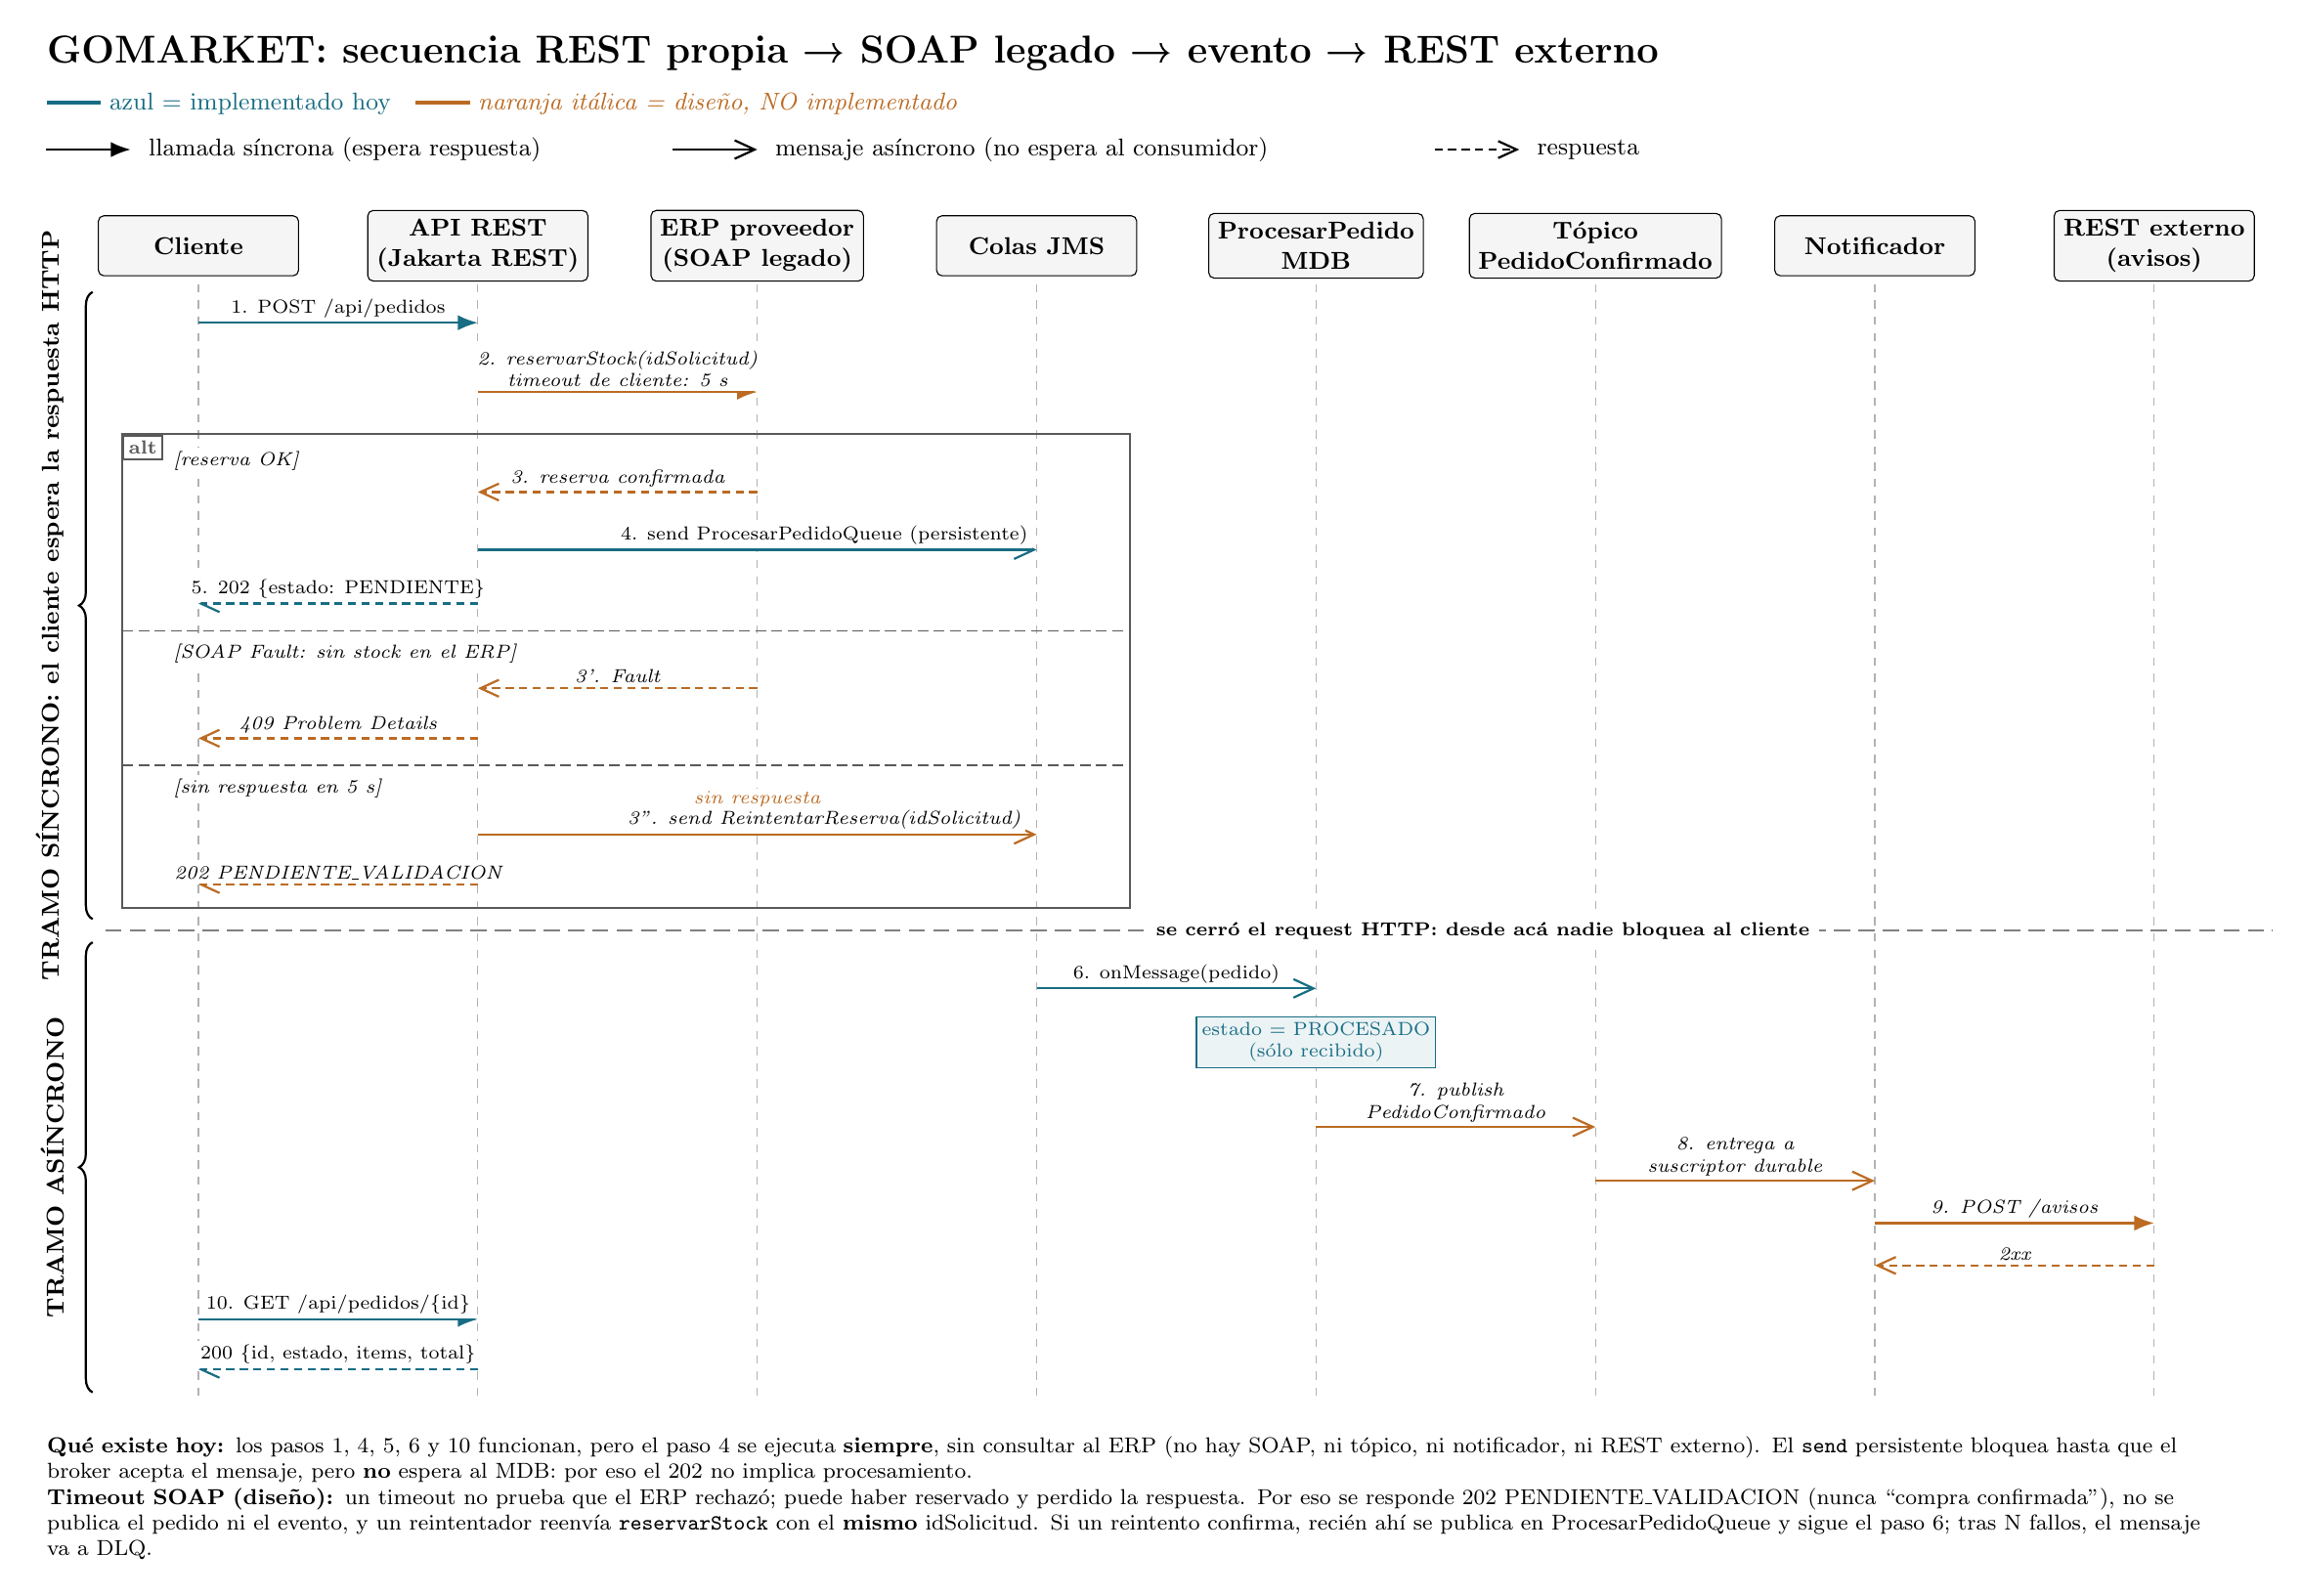
\begin{tikzpicture}[x=1.1cm,y=1cm,
  actor/.style={draw,rounded corners=2pt,fill=gray!8,align=center,
                minimum width=2.6cm,minimum height=0.78cm,font=\small\bfseries},
  % UML: llamada síncrona = punta llena; mensaje asíncrono = punta abierta;
  % respuesta = línea punteada.
  sinc/.style={-{Latex[length=2.6mm,width=2mm]},thick},
  asinc/.style={-{Straight Barb[length=2.6mm,width=2.4mm]},thick},
  resp/.style={-{Straight Barb[length=2.4mm,width=2.2mm]},thick,dash pattern=on 3pt off 2pt},
  imp/.style={draw=real},
  dis/.style={draw=futuro},
  et/.style={font=\scriptsize,fill=white,inner sep=1.5pt,align=center},
  etd/.style={et,font=\scriptsize\itshape},
  guarda/.style={font=\scriptsize\itshape,anchor=west,fill=white,inner sep=1.5pt}]

% ---------- título y leyenda ----------
\node[font=\Large\bfseries,anchor=west] at (-1.9,2.5)
  {GOMARKET: secuencia REST propia → SOAP legado → evento → REST externo};
\node[font=\small,anchor=west] at (-1.9,1.85) {%
  \textcolor{real}{\rule[0.5ex]{7mm}{1.4pt}~azul = implementado hoy}\quad
  \textcolor{futuro}{\rule[0.5ex]{7mm}{1.4pt}~\textit{naranja itálica = diseño, NO implementado}}};
\draw[sinc] (-1.8,1.25) -- (-0.8,1.25);
\node[font=\small,anchor=west] at (-0.7,1.25) {llamada síncrona (espera respuesta)};
\draw[asinc] (5.6,1.25) -- (6.6,1.25);
\node[font=\small,anchor=west] at (6.7,1.25) {mensaje asíncrono (no espera al consumidor)};
\draw[resp] (14.6,1.25) -- (15.6,1.25);
\node[font=\small,anchor=west] at (15.7,1.25) {respuesta};

% ---------- participantes ----------
\foreach \x/\nombre in {0/Cliente,3.3/API REST\\(Jakarta REST),6.6/ERP proveedor\\(SOAP legado),
                        9.9/Colas JMS,13.2/ProcesarPedido\\MDB,16.5/Tópico\\PedidoConfirmado,
                        19.8/Notificador,23.1/REST externo\\(avisos)}{
  \node[actor] at (\x,0) {\nombre};
  \draw[gray!60,dashed] (\x,-0.5) -- (\x,-15.0);
}

% ---------- tramos ----------
\draw[decorate,decoration={brace,amplitude=5pt,mirror},thick] (-1.25,-0.6) -- (-1.25,-8.75)
  node[midway,left=7pt,rotate=90,anchor=south,font=\small\bfseries] {TRAMO SÍNCRONO: el cliente espera la respuesta HTTP};
\draw[decorate,decoration={brace,amplitude=5pt,mirror},thick] (-1.25,-9.05) -- (-1.25,-14.9)
  node[midway,left=7pt,rotate=90,anchor=south,font=\small\bfseries] {TRAMO ASÍNCRONO};
\draw[gray,thick,dash pattern=on 6pt off 3pt] (-1.1,-8.9) -- (24.5,-8.9);
\node[font=\scriptsize\bfseries,fill=white,anchor=west] at (11.2,-8.9) {se cerró el request HTTP: desde acá nadie bloquea al cliente};

% 1. entrada REST (real)
\draw[sinc,imp] (0,-1.0) -- node[et,above] {1. POST /api/pedidos} (3.3,-1.0);
% 2. SOAP (diseño)
\draw[sinc,dis] (3.3,-1.9) -- node[etd,above] {2. reservarStock(idSolicitud)\\timeout de cliente: 5 s} (6.6,-1.9);

% ---------- alt ----------
\draw[thick,gray!70!black] (-0.9,-2.45) rectangle (11.0,-8.6);
\node[draw,thick,gray!70!black,fill=white,font=\scriptsize\bfseries,anchor=north west,
      inner sep=2pt] at (-0.9,-2.45) {alt};
\node[guarda] at (-0.35,-2.8) {[reserva OK]};
\draw[resp,dis] (6.6,-3.2) -- node[etd,above] {3. reserva confirmada} (3.3,-3.2);
\draw[asinc,imp] (3.3,-3.95) -- node[et,above,pos=0.62] {4. send ProcesarPedidoQueue (persistente)} (9.9,-3.95);
\draw[resp,imp] (3.3,-4.65) -- node[et,above] {5. 202 \{estado: PENDIENTE\}} (0,-4.65);

\draw[gray!70!black,dash pattern=on 4pt off 2pt] (-0.9,-5.0) -- (11.0,-5.0);
\node[guarda] at (-0.35,-5.3) {[SOAP Fault: sin stock en el ERP]};
\draw[resp,dis] (6.6,-5.75) -- node[etd,above] {3'. Fault} (3.3,-5.75);
\draw[resp,dis] (3.3,-6.4) -- node[etd,above] {409 Problem Details} (0,-6.4);

\draw[gray!70!black,dash pattern=on 4pt off 2pt] (-0.9,-6.75) -- (11.0,-6.75);
\node[guarda] at (-0.35,-7.05) {[sin respuesta en 5 s]};
\node[font=\scriptsize\itshape,text=futuro,fill=white,inner sep=1pt] at (6.6,-7.2) {sin respuesta};
\draw[asinc,dis] (3.3,-7.65) -- node[etd,above,pos=0.62] {3''. send ReintentarReserva(idSolicitud)} (9.9,-7.65);
\draw[resp,dis] (3.3,-8.3) -- node[etd,above] {202 PENDIENTE\_VALIDACION} (0,-8.3);

% ---------- tramo asíncrono ----------
\draw[asinc,imp] (9.9,-9.65) -- node[et,above] {6. onMessage(pedido)} (13.2,-9.65);
\node[draw=real,fill=real!8,font=\scriptsize,align=center,inner sep=2pt,text=real]
  at (13.2,-10.35) {estado = PROCESADO\\(sólo recibido)};
\draw[asinc,dis] (13.2,-11.45) -- node[etd,above] {7. publish\\PedidoConfirmado} (16.5,-11.45);
\draw[asinc,dis] (16.5,-12.15) -- node[etd,above] {8. entrega a\\suscriptor durable} (19.8,-12.15);
\draw[sinc,dis] (19.8,-12.7) -- node[etd,above] {9. POST /avisos} (23.1,-12.7);
\draw[resp,dis] (23.1,-13.25) -- node[etd,above] {2xx} (19.8,-13.25);
\draw[sinc,imp] (0,-13.95) -- node[et,above] {10. GET /api/pedidos/\{id\}} (3.3,-13.95);
\draw[resp,imp] (3.3,-14.6) -- node[et,above] {200 \{id, estado, items, total\}} (0,-14.6);

% ---------- nota ----------
\node[font=\footnotesize,anchor=north west,text width=28cm,align=left] at (-1.9,-15.35) {%
  \textbf{Qué existe hoy:} los pasos 1, 4, 5, 6 y 10 funcionan, pero el paso 4 se ejecuta
  \textbf{siempre}, sin consultar al ERP (no hay SOAP, ni tópico, ni notificador, ni REST externo).
  El \texttt{send} persistente bloquea hasta que el broker acepta el mensaje, pero
  \textbf{no} espera al MDB: por eso el 202 no implica procesamiento.\\
  \textbf{Timeout SOAP (diseño):} un timeout no prueba que el ERP rechazó; puede haber reservado y
  perdido la respuesta. Por eso se responde 202 PENDIENTE\_VALIDACION (nunca ``compra
  confirmada''), no se publica el pedido ni el evento, y un reintentador reenvía
  \texttt{reservarStock} con el \textbf{mismo} idSolicitud. Si un reintento confirma, recién ahí
  se publica en ProcesarPedidoQueue y sigue el paso 6; tras N fallos, el mensaje va a DLQ.};
\end{tikzpicture}
\end{document}
